\documentclass[10pt]{article}
\usepackage[polish]{babel}
\usepackage[utf8]{inputenc}
\usepackage[T1]{fontenc}
\usepackage{amsmath}
\usepackage{amsfonts}
\usepackage{amssymb}
\usepackage[version=4]{mhchem}
\usepackage{stmaryrd}
\usepackage{graphicx}
\usepackage[export]{adjustbox}
\graphicspath{ {./images/} }

\title{GIMNAZJUM }

\author{}
\date{}


\begin{document}
\maketitle
\begin{enumerate}
  \item Rozwiąż w liczbach całkowitych równanie
\end{enumerate}

\[
x \cdot y \cdot(x+2017 y)=2017^{2017}
\]

\begin{enumerate}
  \setcounter{enumi}{1}
  \item Dane są dwa kwadraty, jeden przy drugim, o bokach \(a\) i \(b\). Wyznacz stosunek pól: zamalowanej części dużego kwadratu i tegoż kwadratu.\\
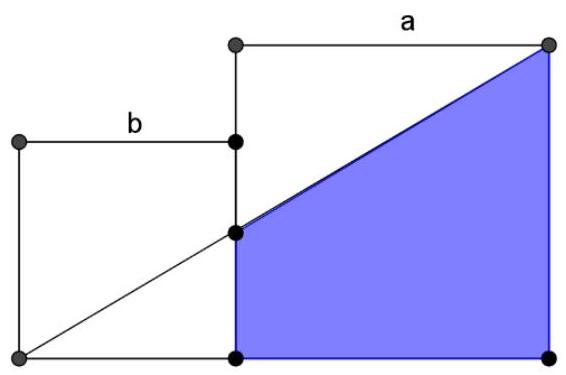
\includegraphics[max width=\textwidth, center]{2024_11_21_6a4ec3a704d41ae8fcd4g-1}
  \item Wiadomo, że \(x+\frac{1}{x}=12\). Ile wynosi \(x^{2}+\frac{1}{x^{2}}\) ?
\end{enumerate}

\section*{LICEUM}
\begin{enumerate}
  \item Współczynniki \(\mathrm{a}, \mathrm{b}, \mathrm{c}, \mathrm{d}\) wielomianu \(W(x)=x^{4}+a x^{3}+b x^{2}+c x+d\) są liczbami całkowitymi nieparzystymi. Udowodnić, że wielomian ten nie posiada pierwiastków całkowitych.
  \item Wykaż, że liczba \(3^{54}-3^{27} \cdot 2^{12}+2^{24}\) jest złożona.
  \item W czworokącie wypukłym środki boków połączono z wierzchołkami tak, jak na rysunku. Udowodnij, że pole czerwonego czworokąta jest równe sumie pól niebieskich trójkątów.\\
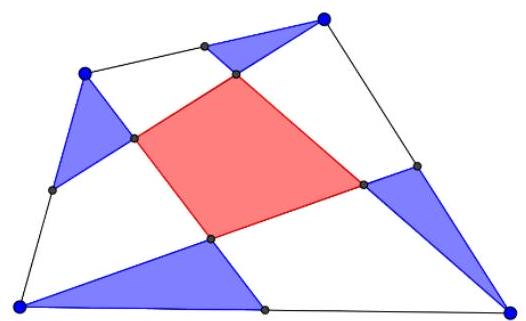
\includegraphics[max width=\textwidth, center]{2024_11_21_6a4ec3a704d41ae8fcd4g-1(1)}
\end{enumerate}

\end{document}